\documentclass[a4paper, Arial, 12pt]{article}

\usepackage[brazil]{babel}
\usepackage[utf8]{inputenc}
\usepackage{hyperref} % criar hyperlinks
\usepackage{listings} % utilizado para dar highlight em código
\usepackage[dvipsnames]{xcolor}
\usepackage{graphicx} % importar imagens
\usepackage[export]{adjustbox}

\lstdefinestyle{customc}{ %custom color para código do arduino
  belowcaptionskip=1\baselineskip,
  backgroundcolor=\color{lightgray},
  breaklines=true,
  frame=single,
  xleftmargin=\parindent,
  language=C,
  showstringspaces=false,
  basicstyle=\footnotesize\ttfamily,
  keywordstyle=\bfseries\color{ForestGreen},
  commentstyle=\itshape\color{darkgray},
  identifierstyle=\color{blue},
  stringstyle=\color{gray},
  breaklines=true,
  morekeywords={bool},
}

\title{Etapas e dificuldades}
\author{Victor Vieira Paulino
\and
Arthur Cicuto Pires}
\date{\today}

\begin{document}

\maketitle

\section{Módulo do Ônibus}

\subsection{Hardware}

\begin{enumerate}
\item HM-10 - Bluetooth 4.0 BLE module
\item Arduino Uno
\end{enumerate}

Arduino Uno é utilizado apenas como ponte para configurar o módulo HM-10. A ligação deve seguir o diagrama abaixo.

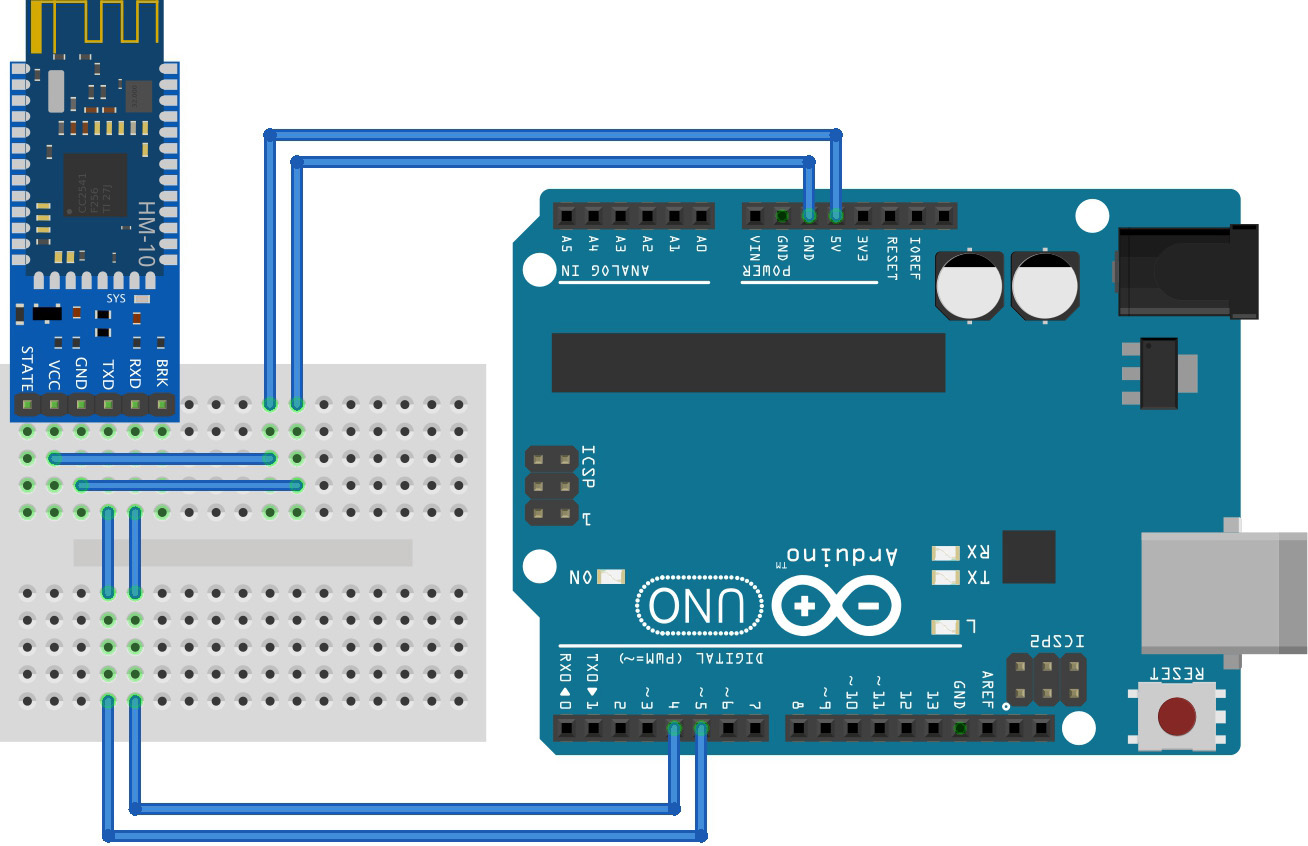
\includegraphics[width=10cm, center]{images/arduino-hm10}

\subsection{Software}

\begin{itemize}
\item Arduino IDE 1.8.3 ou superior. 
\end{itemize}

\subsection{Configuração}

Conecte o arduino Uno ao computador e compile o código abaixo utilizando a IDE do arduino.

\lstinputlisting[style=customc]{codes/arduino-code.ino}

Após compilador, utilizando o Serial Monitor da IDE, execute os comandos AT na seguinte ordem:

Obs: Quanto menor o tempo de envio, maior a economia de energia.

\begin{enumerate}
\item AT+RENEW //Coloca nos padrões de fábrica
\item AT+RESET //Reinicia para aplicar os padrões de fábrica
\item AT+MARJ0xNNNN //Define o valor Marjor
\item AT+MINO0xNNNN //Define o valor Minor
\item AT+NAMEMeuBeacon //Define o nome do Beacon
\item AT+ADVI5 //Define tempo de envio. 5 = 546.25 millisegundos
\item AT+ADTY3 //Define como não pareável
\item AT+IBEA1 //Habilita como Beacon
\item AT+DELO2 //Configura para apenas emitir sinal
\item AT+PWRM0 //Habilita auto-sleep para economizar energia
\item AT+RESET
\end{enumerate}


Após configurado, pode ser ligado em uma bateria 3v para utilização.

\subsection{Referências}

\href{ftp://imall.iteadstudio.com/Modules/IM130614001_Serial_Port_BLE_Module_Master_Slave_HM-10/DS_IM130614001_Serial_Port_BLE_Module_Master_Slave_HM-10.pdf}{HM-10 Bluetooth 4.0 BLE module Datasheet}
\\
\href{https://www.arduino.cc/en/main/software}{Arduino IDE}
\\
\href{https://github.com/metractive/beacon-study}{Repositório da Metractive - Como construir Beacons}

\section{Módulo do ponto de ônibus}

teste

\section{Aplicativo}

teste

\section{Web service}

Falar sobre o MEAN stack e sobre as dificuldades que estou encontrando sobre como trabalhar com cada tecnologia da pilha.

\end{document}